

Phase-2 upgrades of CMS subsytems including the replacement of the tracker, barrel ECAL and DT front-end electronics, and forward calorimeters, will be given priority during LS3. These projects require prolonged access to the CMS inner barrel and YE1 disks, so throughout LS3, CMS will remain in a configuration with both endcaps open away from the barrel. This will prevent access to the YE2 and YE3 disks on which CSCs in stations 1, 2, and 3 are mounted. Therefore, Phase-2 upgrades of the CSCs requiring the removal of chambers in those stations was scheduled for LS2, when the YE disks could be spaced apart. Upgrades of on-chamber CSC electronics would be given preference during LS2, while replacement of boards off-chamber in the peripheral crates will wait to be upgraded until LS3. Other upgrades during LS2 included Phase-1 upgrades to the HCAL and the installation of new Phase-2 GEM detectors. The full schedule of LS2 activity for CSCs upgrades followed a highly-optimized timetable of parallel chamber extraction, refurbishment, testing, installation, and commisioning of all 180 MEx/1 chambers, to be completed in just 60 weeks. The timetable was divided into four staggered workstreams based on chamber type: 1. ME+1/1, 2. ME+234/1, 3. ME-1/1, and 4. ME-234/1. Excellent progress at approximately two chambers per day was sustained throughout 2019 with workstreams 1-3, however, the outbreak of the Covid-19 pandemic presented significant setbacks to workflow and manpower, causing delays toward the end of LS2. In response, the CSC team made every effort to finish the upgrades as quickly and safely as possible, and despite a two-and-a-half month shift and a two month extension of the 4th work stream, by 2021 all CSC upgrade activity had succesfully concluded in time for Run 3 preparations.

\subsection{Chamber extraction} \label{sec:ChamberExtraction}

One at a time, chambers were disconnected from water, gas, and cabling before they were be detached from the endcap yokes. Once dismounted, CSCs were brought to the surface with an overhead crane. Inside the surface building SX5 is a CSC facility where refurbishment and testing sites are located. Extracted chambers were placed horizontally on rolling tables for in situ refurbishment and transport to each testing site within the CSC facility, while a backlog of chambers awaiting refurbishment or installation were kept vertically on storage cradles. Extraction began with the ME1/1 chambers so their DCFEBs could be harvested for the ME234/1 chambers, but parallel testing sites allowed both types to undergo refurbishment and testing simultaneously. A photograph of the CSC facility in SX5 is shown in Fig.~\ref{fig:SX5}.

\begin{figure}[H]
    \centering
    \includegraphics[width=1\textwidth]{Images/Phase2Upgrades/CSCactivity/SX5Lab.png}
    \caption{An aerial view of the CSC facility in SX5 used for the Phase-2 refurbishment and testing of CSC modules during LS1 and LS2.}
    \label{fig:SX5}
\end{figure}

\subsection{DCFEB temperature study} \label{sec:DCFEBTemperatureStudy}
The on-chamber electronics boards mounted to the face of each CSC generate a significant amount of heat while operating, a load of roughly \SI{70}{W} per chamber, and need a cooling system to prevent overheating. Beneath the (D)CFEBs, ALCTs, LVDB(5)s, and AFEBs, are copper plates, with a continuous 1/4'' copper tube brazed to each plate. Thermal pads are layered on each electronics component (ASICs, FPGAs, etc.) to provide good thermal contact with the copper plates, efficiently carrying heat away from the electronics. A photograph of a cooling cover and thermal pad strips for a DCFEB is shown in Fig.~\ref{fig:CoolingCover}. A pressurized water system flows through each chamber's copper loop and cools the plates. The supply and return ends of each chamber's copper pipe are connected via flexible hosing to neighboring CSCs forming three-chamber circuits, which are then connected to a larger cooling manifold secured to each YE disk, allowing water to flow through all the CSCs. Input water temperature is approximately 18-\SI{20}{\celsius} and is optimized to limit the temperature rise per connection to \SI{2}{\celsius}.

\begin{figure}[H]
    \centering
    \includegraphics[width=1\textwidth]{Images/Phase2Upgrades/DCFEBTempStudy/DCFEBpadding.png}
    \caption{}
    \label{fig:CoolingCover}
\end{figure}

To validate that the cooling system on ME234/1 chambers is sufficient to cool the DCFEBs that will replace the CFEBs, the efficiency of the thermal-pad-to-cooling-plate configuration was studied. An ME3/1 chamber refurbished with DCFEBs was connected to cooling and LV power using one of the FAST sites in the CSC lab at SX5 (see Sec.~\ref{sec:ChamberTesting}). With the power supply on and the DCFEBs left idle, the temperature of each DCFEBs' FPGA (using a built-in thermometer) was collected via a web-based monitor (the so-called ``yellow page'') on a minute-by-minute basis in half-hour sessions. The cooling efficiency of several configurations were studied by varying the thermal pad thickness, DCFEB location on-chamber, and type of copper cooling cover. 

It was observed that that FPGAs exibit a large temperature variation, roughly a \SI{10}{\celsius} range between DCFEBs. By swapping the location of two of the five DCFEBs on the chamber, which are arranged side-by-side, it was established that the temperature variations were an artifact of each DCFEB and that the cooling system provides a homogenous temperature map accross the DCFEBs, shown in Figs.~\ref{fig:FPGAtemp1}-\ref{fig:FPGAtemp2}. The rise in temperature of FPGA 466 in the right-hand plot of Fig.~\ref{fig:FPGAtemp1} was due to poor thermal contact with the cooling cover. DCFEBs (and CFEBs) are not actually mounted to the cooling baseplate, rather, they are secured to copper cooling covers, offset with \SI{5.0}{mm} stand-offs, and the cover is screwed to the baseplate. It is the cover that the FPGAs (and most other electronics) are in thermal contact with, while strips of thermal padding between the cover and the baseplate carry heat from the cover to the cooling system. By removing the threading in the holes of the cover it can be screwed down closer to the baseplate, providing better thermal contact, and reducing the overall temperature of the FPGAs (see Fig.~\ref{fig:FPGAtemp2}). A later study revealed that \SI{1.5}{mm}-thick thermal pads provided better thermal contact over \SI{1.0}{mm}-thick thermal pads.

\begin{figure}[H]
    \centering
    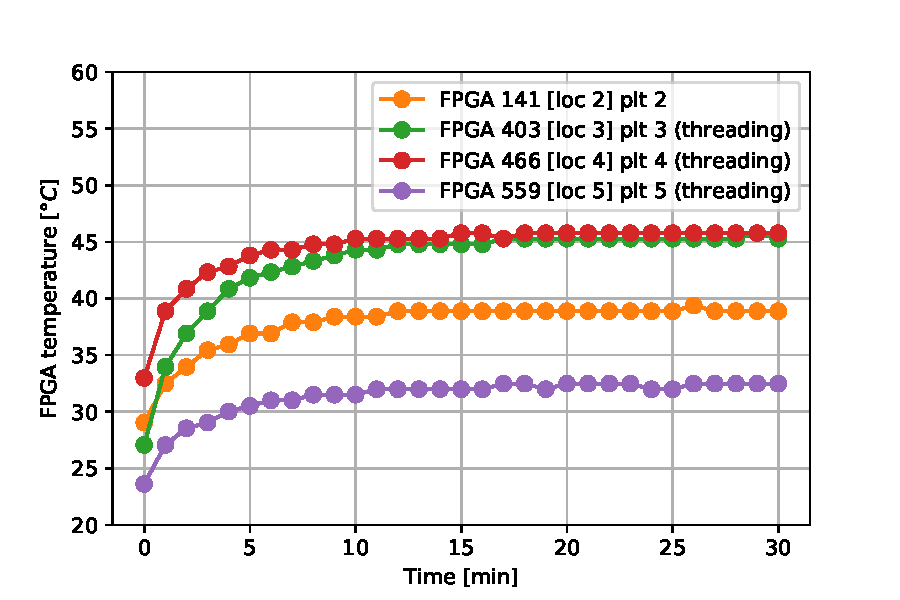
\includegraphics[width=0.49\textwidth]{Images/Phase2Upgrades/DCFEBTempStudy/TempPlot_2019_01_14_plot1-5295.pdf}
    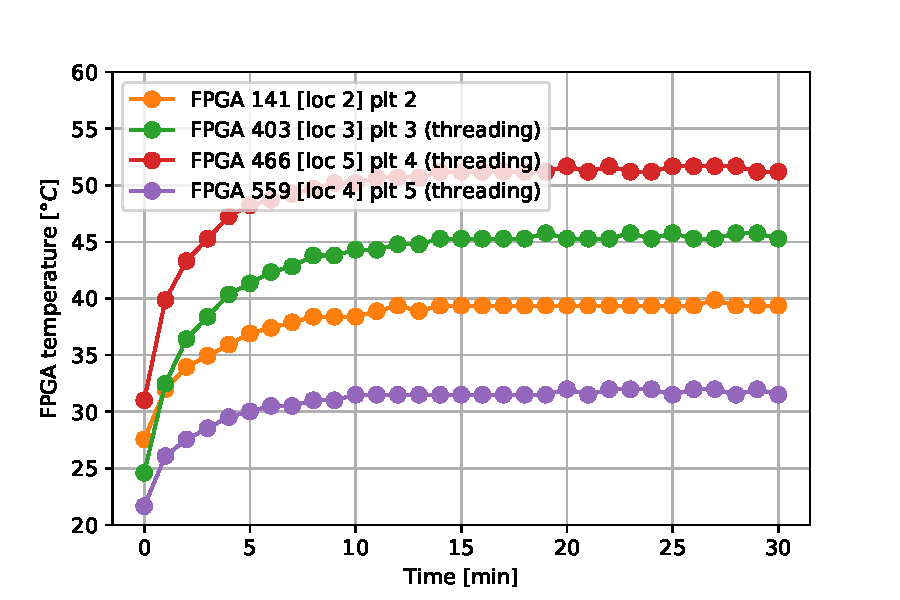
\includegraphics[width=0.49\textwidth]{Images/Phase2Upgrades/DCFEBTempStudy/TempPlot_2019_01_14_plot2-5296.pdf}
    \caption{FPGA temperature sampled every minute of five idle DCFEBs on an ME3/1 CSC. The location on-chamber of DCFEBs 466 and 559 have been swapped betweeen the two plots. The cooling plates on DCFEBs 403, 466, and 559 have threading.}
    \label{fig:FPGAtemp1}
\end{figure}

\begin{figure}[H]
    \centering
    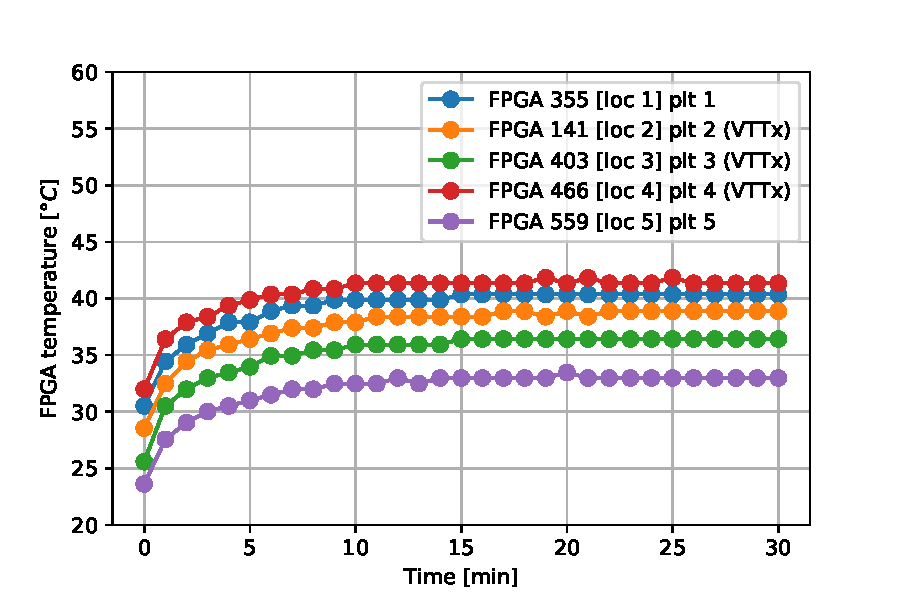
\includegraphics[width=0.49\textwidth]{Images/Phase2Upgrades/DCFEBTempStudy/TempPlot_2019_01_17_nothread12345-5433.pdf}
    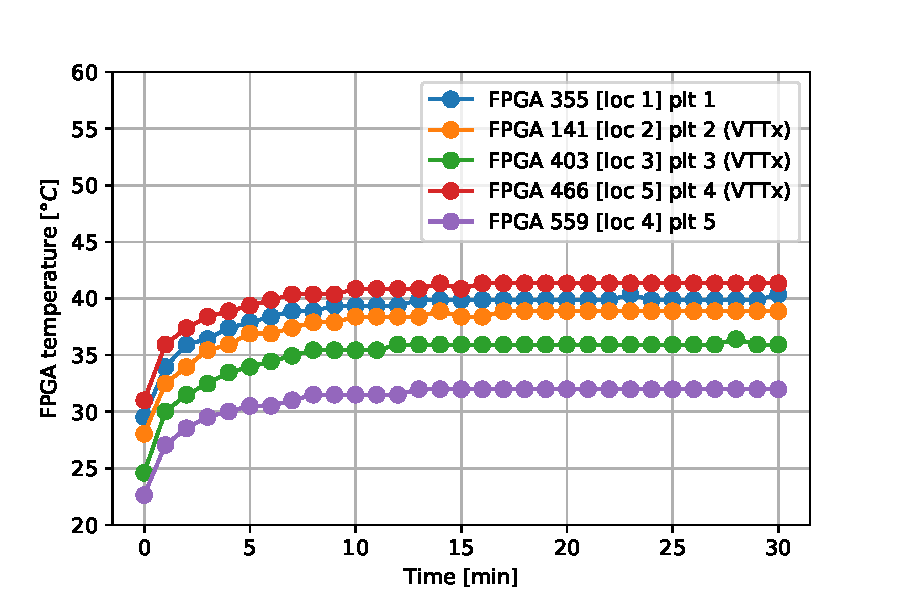
\includegraphics[width=0.49\textwidth]{Images/Phase2Upgrades/DCFEBTempStudy/TempPlot_2019_01_17_nothread12354-5430.pdf}
    \caption{FPGA temperature sampled every minute of five idle DCFEBs on an ME3/1 CSC. The location on-chamber of DCFEBs 466 and 559 have been swapped betweeen the two plots. The cooling plates on all DCFEBs have no threading.}
    \label{fig:FPGAtemp2}
\end{figure}

\subsection{ME1/1 refurbishment} \label{sec:ME1/1refurbishment}

Refurbishment of each chamber was performed by a dedicated team: roughly 20 CSC group members comprised of post-docs, graduate students, and some undergraduate students, all of whom received training in the assembly and disassembly for both ME1/1 and ME234/1 chambers, as the construction and placement of the on-chamber electronics are somewhat different between the two chamber types. Chambers were refurbished at the CSC lab in SX5, following a detailed checklist. The refurbishment procedure of the ME1/1 chambers during LS2 was modeled after the ME1/1 upgrade program from LS1. A rough outline of the steps required to upgrade each electronic component is: 

\begin{itemize}
    \item LVDB7:
    \begin{enumerate}
        \item LVDB7 cover is removed and inspected for any damage
        \item LVDB7 cover is reattached (no LVDB upgrades on ME1/1)
    \end{enumerate}
    \item xDCFEBs:
    \begin{enumerate}
        \item DCFEB covers are removed, and strip cables, LV cables, and patch cables (connecting CFEBs together) are all disconnected
        \item Starting from the top of the chamber, and working down, all seven DCFEBs are unscrewed, removed, serialized and dated, and taken to temporary storage following radiation-safe guidelines
        \item Clean xDCFEBs covers with ethanol, cut and place thermal pads onto covers
        \item New xDCFEBs are installed, screwed down, and reconnected to strip, LV, and patch cables
        \item DCFEB covers are reattached
    \end{enumerate}
    \item ALCT-LX100:
    \begin{enumerate}
        \item ALCT-S6 cover is removed and all cables disconnected
        \item ALCT-S6 mezzanine is removed
        \item Thermal block with thermal pad placed on baseboard
        \item New ALCT-LX100 inserted gently to connector and secured
    \end{enumerate}
\end{itemize}

\subsection{ME234/1 refurbishment} \label{sec:ME234/1refurbishment}

As each ME1/1 chamber was refurbished, the DCFEBs harvested from that chamber were taken off-site to have their VTTx adapter boards installed. After the DCFEBs returned to the CSC lab in SX5, refurbishment of the ME234/1 chambers was carried out by the refurbishment team in situ, following a checklist similar to that used for ME1/1 chambers. The procedure is as follows: 

\begin{itemize}
    \item LVDB5:
    \begin{enumerate}
        \item LVDB cover, LVMB mezzanine, and thermal pads are removed
        \item LVDB baseboard is unscrewed and barcodes are applied to LVDB baseboard and LVMB mezzanine
        \item New thermal padding is cut and applied to LVDB5 baseboard
        \item New LVDB5 baseboard is installed and screwed down
        \item LVMB mezzanine is installed
    \end{enumerate}
    \item DCFEBs:
    \begin{enumerate}
        \item CFEB cover and individual cooling plates are removed, and strip cables, LV cables, and patch cables (connecting CFEBs together) are all disconnected
        \item All five CFEBs are unscrewed, removed, serialized and dated, and taken to storage following radiation-safe guidelines
        \item DCFEBs harvested from ME1/1 chambers are installed, screwed down, and reconnected to strip, LV, and patch cables
        \item DCFEB cooling plates and covers are reattached
    \end{enumerate}
    \item ALCT-LX150T:
    \begin{enumerate}
        \item ALCT mezzanine is removed
        \item Thermal block with thermal pad placed on baseboard
        \item New ALCT-LX150T inserted gently to connector and secured
    \end{enumerate}
    \item Optical fibers:
    \begin{enumerate}
        \item LC connectors on the optical fiber fan-out are connected to each DCFEB and ALCT, while the MTP connector is secured to the side of the chamber (more info on the optical fibers in Sec.~\ref{sec:OpticalFibers})
    \end{enumerate}
\end{itemize}

\subsection{Chamber testing} \label{sec:ChamberTesting}

Once a CSC has been refurbished but prior to reinstallation, it undergoes a series of tests designed to load firmware, validate the performance of the newly installed electronics, and identify any mistakes made during refurbishement. Chamber testing prior to reinstallation is a three-stage process: initial testing at the Final Assembly and System Testing (FAST) site, long-term testing at the Long-Term Testing (LTT) site, and final testing again at the FAST site. Both FAST and LTT sites are located inside the CSC lab at SX5 and consist of parallel testing stands (FAST 1 and FAST 2; LTT 1, LTT 2, and a third ME1/1-dedicated LTT stand) that allow 2-3 chambers to efficiently undergo testing simultaniously. A photograph of the author inspecting a CSC at the FAST testing sites in SX5 is shown in Fig.~\ref{fig:FAST}.

\begin{figure}[H]
    \centering
    \includegraphics[width=1\textwidth]{Images/Phase2Upgrades/CSCactivity/FASTsites.png}
    \caption{FAST test stands at the CSC facility in SX5. An ME1/1 chamber undergoing testing is connected to one FAST site (left-hand-side of photo), while the author inspects an ME2/1 chamber connected to the other FAST site (middle of photo).}
    \label{fig:FAST}
\end{figure}

The FAST sites are equipped to supply each CSC with high and low voltage, gas, cooling, and trigger and data links to a dedicated peripheral crate. After connecting the chamber to power, high voltage supply, trigger/DAQ readout cables to OTMB and ODMB, and both gas and water supplies, the (x)DCFEB and ALCT mezzanine firmware is uploaded and the trigger timing is synchronized. Next, a comprehensive assessment of the health of a CSC's on-chamber electronics is conducted with a suite of tests called the System Test of Endcap Peripheral crates and chamber electronics (STEP) . The STEP tests follow the sequence:
\begin{itemize}
    \item AFEB threshold and analog noise
    \item AFEB connectivity and crosstalk
    \item AFEB counting noise
    \item ALCT-AFEB time delay
    \item CFEB pedestals
    \item CFEB connectivity
    \item CFEB pulse shape and crosstalk
    \item CFEB gain
    \item Comparator thresholds and analog noise
    \item Comparator logic
    \item ALCT trigger
    \item High-statistics cosmics
\end{itemize}

Typically, all the FAST testing, including the STEP tests, takes about six hours to perform for two chambers in parallel. However, when problems with the electronics are revealed, it can take up to a day of debugging until the chamber again passes all testing at the FAST site. Common issues revealed from FAST tests include connection issues (usually fixed with reseating cables), problematic electronic boards (requires examination, repair, or replacement by experts), and chamber problems like shorted strips, broke, wires, etc., which are noted but left alone.

After finishing the STEP tests, chambers are brought to the neighboring LTT sites for 48-hour monitoring. The LTT stands supply the chambers with low voltage, gas, and cooling---no high voltage is needed. Voltage, current, and temperature stability are all monitored for a minimum of 48 hours, finishing with the low voltage portion of the STEP tests. Finally, two hours of post-LTT tests back at the FAST sites reveal if there are any gas leaks.

\subsection{Chamber installation and commissioning} \label{sec:CSCInstallationAndCommissioning}

Immediately following refurbishment and testing, each CSC was lowered back down into the experimental cavern (UXC) to be reinstalled on CMS. Chambers are reinstalled onto the YE disks in nearly the same way they are extracted, however, prior to connecting gas, water, and HV---with only LV to power the electronics---the chambers undergo initial testing of connectivity and mapping. Next, the on-board clocks of the electronics for each CSC must be configured with respect to each other to account for differences in location and cable length. After reconnecting all services, the chambers are commissioned by recording cosmic rays. Following succesfull commissioning, the upgraded CSCs are integrated with the rest of CMS and the global DAQ system, where the chambers can participate in global data taking. Hit occupancy and timing plots allow the overall functioning of the CSCs to be monitored.

